\documentclass{article}
\usepackage{amsmath}
\usepackage{tikz}
\usetikzlibrary{arrows.meta, decorations.pathreplacing, positioning}

\begin{document}

\[
\mathcal{Z}(\boldsymbol{q}) =
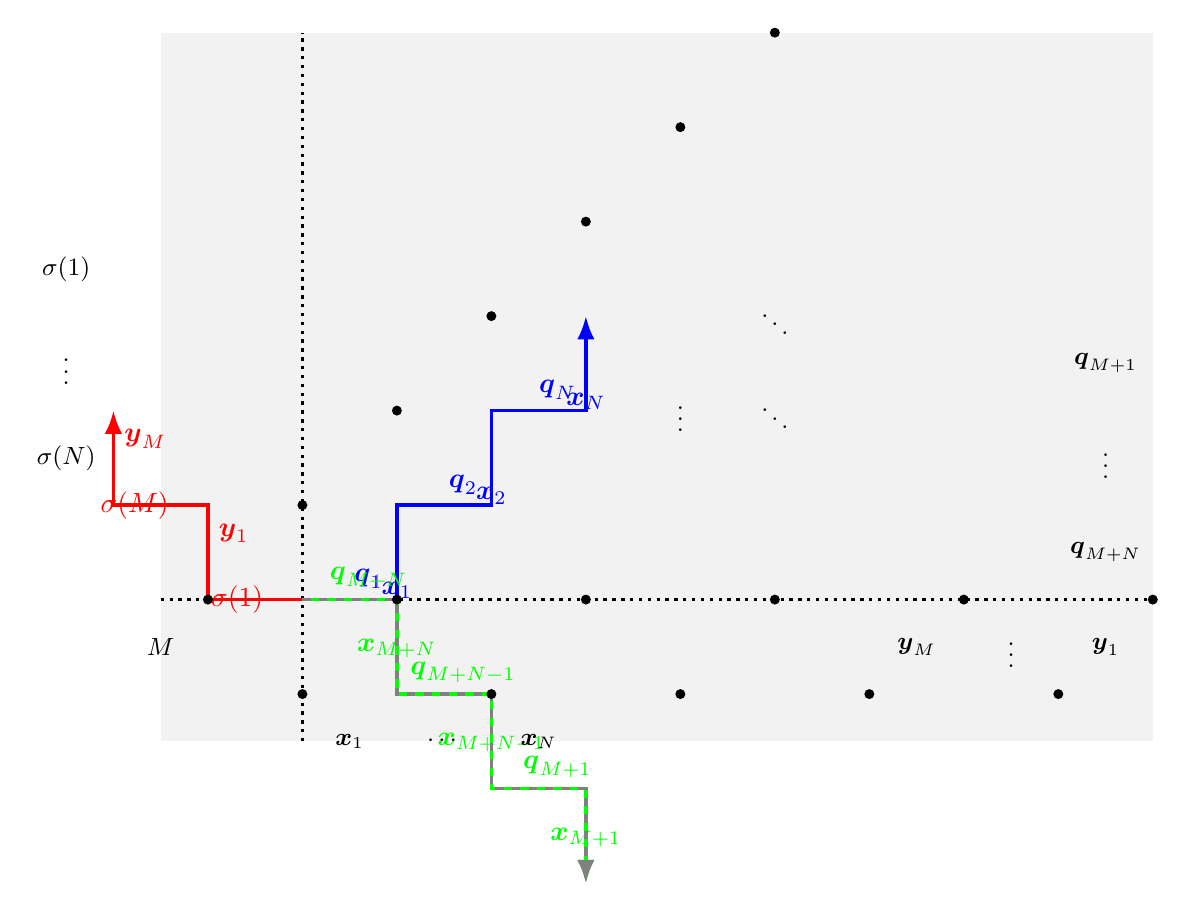
\begin{tikzpicture}[baseline=(current bounding box.center), scale=1.2]
    % Define styles for arrows
    \tikzset{
        >=Latex,
        arrow/.style={->, very thick},
        dashedarrow/.style={->, dashed, very thick},
        dotline/.style={dotted, gray!50, thin},
        label/.style={font=\small, black}
    }

    % Draw the grid and shading
    \foreach \i in {1,...,6} {
        \draw[dashed, gray!50] (-1.5, \i-0.5) -- (9, \i-0.5);
        \draw[dashed, gray!50] (\i-0.5, -1.5) -- (\i-0.5, 6);
    }
    \fill[gray!10] (-1.5,-1.5) rectangle (9,6);

    % Draw the vertical and horizontal lines
    \draw[very thick, dotted] (-1.5, 0) -- (9, 0); % Horizontal line at y=0
    \draw[very thick, dotted] (0, -1.5) -- (0, 6); % Vertical line at x=0

    % Draw the blue path
    \draw[blue, arrow] (0, 0) -- node[above, pos=0.7] {$\boldsymbol{q}_1$} ++(1, 0)
                       -- node[below, pos=0.3] {$\boldsymbol{x}_1$} ++(0, 1)
                       -- node[above, pos=0.7] {$\boldsymbol{q}_2$} ++(1, 0)
                       -- node[below, pos=0.3] {$\boldsymbol{x}_2$} ++(0, 1)
                       -- node[above, pos=0.7] {$\boldsymbol{q}_N$} ++(1, 0)
                       -- node[below, pos=0.3] {$\boldsymbol{x}_N$} ++(0, 1);

    % Draw the red path
    \draw[red, arrow] (0, 0) -- node[left, pos=0.3] {$\sigma(1)$} ++(-1, 0)
                      -- node[right, pos=0.7] {$\boldsymbol{y}_1$} ++(0, 1)
                      -- node[left, pos=0.3] {$\sigma(M)$} ++(-1, 0)
                      -- node[right, pos=0.7] {$\boldsymbol{y}_M$} ++(0, 1);

    % Draw the green path
    \draw[green, arrow] (0, 0) -- node[above, pos=0.7] {$\boldsymbol{q}_{M+N}$} ++(1, 0)
                        -- node[below, pos=0.3] {$\boldsymbol{x}_{M+N}$} ++(0, -1)
                        -- node[above, pos=0.7] {$\boldsymbol{q}_{M+N-1}$} ++(1, 0)
                        -- node[below, pos=0.3] {$\boldsymbol{x}_{M+N-1}$} ++(0, -1)
                        -- node[above, pos=0.7] {$\boldsymbol{q}_{M+1}$} ++(1, 0)
                        -- node[below, pos=0.3] {$\boldsymbol{x}_{M+1}$} ++(0, -1);

    % Draw the gray path
    \draw[gray, dashedarrow] (0, 0) -- ++(1, 0)
                             -- ++(0, -1)
                             -- ++(1, 0)
                             -- ++(0, -1)
                             -- ++(1, 0)
                             -- ++(0, -1);

    % Add additional labels
    \node[label] at (-1.5, -0.5) {$M$};
    \node[label] at (8.5, 0.5) {$\boldsymbol{q}_{M+N}$};
    \node[label] at (8.5, 1.5) {$\vdots$};
    \node[label] at (8.5, 2.5) {$\boldsymbol{q}_{M+1}$};

    \node[label] at (0.5, -1.5) {$\boldsymbol{x}_1$};
    \node[label] at (1.5, -1.5) {$\cdots$};
    \node[label] at (2.5, -1.5) {$\boldsymbol{x}_N$};

    \node[label] at (-2.5, 1.5) {$\sigma(N)$};
    \node[label] at (-2.5, 2.5) {$\vdots$};
    \node[label] at (-2.5, 3.5) {$\sigma(1)$};

    \node[label] at (6.5, -0.5) {$\boldsymbol{y}_M$};
    \node[label] at (7.5, -0.5) {$\vdots$};
    \node[label] at (8.5, -0.5) {$\boldsymbol{y}_1$};

    % Add additional annotations
    \node[label] at (4, 2) {$\vdots$};
    \node[label] at (5, 3) {$\ddots$};
    \node[label] at (5, 2) {$\ddots$};

    % Add dots for intersections
    \foreach \x/\y in {-1/0, 0/-1, 1/0, 2/-1, 3/0, 4/-1, 5/0, 6/-1, 7/0, 8/-1, 9/0} {
        \fill (\x, \y) circle (1.5pt);
    }
    \foreach \x/\y in {0/1, 1/2, 2/3, 3/4, 4/5, 5/6} {
        \fill (\x, \y) circle (1.5pt);
    }
\end{tikzpicture}
\]

\end{document}